%Copyright (C) 2022 Wiebke Jahr
%
%This program is free software: you can redistribute it and/or modify
%it under the terms of the GNU Affero General Public License as
%published by the Free Software Foundation, either version 3 of the
%License, or (at your option) any later version.
%
%This program is distributed in the hope that it will be useful,
%but WITHOUT ANY WARRANTY; without even the implied warranty of
%MERCHANTABILITY or FITNESS FOR A PARTICULAR PURPOSE.  See the
%GNU Affero General Public License for more details.
%
%You should have received a copy of the GNU Affero General Public License
%along with this program.  If not, see <https://www.gnu.org/licenses/>.



\documentclass{scrartcl}
\usepackage[english]{babel}
\usepackage{graphicx}
\usepackage{amsmath}
\usepackage{caption}
\usepackage{siunitx}
%\usepackage{natbib}
\usepackage{xspace}
\usepackage{lineno}
\usepackage{csquotes} % needed when bibtex is used with babel in polyglossia (multiple languages)

\usepackage[
	sorting = none, % entries in order they're cited
	citestyle = numeric,
	bibstyle = numeric, %
	%sorting = ydnt, % year (descending), name, title
	backend = biber, %
	hyperref = true, %
	giveninits = true, %
	maxbibnames = 30,
	%date = year, % prints only year from date field
	url = false]{biblatex} %
\renewbibmacro{in:}{}

\usepackage{hyperref}

\linenumbers

\addbibresource{SLMcontrol.bib}

%\graphicspath{{../Figures/}}
\renewcommand{\floatpagefraction}{.8}
\renewcommand{\topfraction}{.8}
\newcommand{\ie}{i.\,e.\xspace}
\newcommand{\Ie}{I.\,e.\xspace}
\newcommand{\eg}{e.\,g.\xspace}
\newcommand{\Eg}{E.\,g.\xspace}
\newcommand{\etc}{etc.\xspace}
\newcommand{\vs}{\emph{vs.}\xspace}
\newcommand{\see}{\emph{cf.}\xspace}
\newcommand{{\na}}{\ensuremath{\mathit{NA}}\xspace}
\newcommand{\ui}[1]{_{\mathrm{#1}}}

\begin{document}
	
	\title{An interactive GUI to control an SLM for STED microscopy and adaptive optics}
	\author{Wiebke Jahr	\\
		\href{mailto:wiebke.jahr@web.de}{wiebke.jahr@web.de}\\
		\url{https://github.com/wiebkejahr/slm\_ control} }
	\maketitle
	
	\section{Rationale}
		%\cite{vanDort2018}: Thesis, otherwise unpublished. Basis of aberrior adaptive optics? iterative correction of coma, spherical, astigmatism
		For several centuries, diffraction of light was believed to fundamentally limit the resolution of light microscopy -- a limit which has since been shattered by various super-resolution microscopies \cite{Hell2015}.
		In theory, the attainable resolution is infinite; yet high light intensities and optical aberrations hinder the separation of fine features \cite{Booth2007,Kubby2013book,Booth2014}.
		
		In STED microscopy, a light pattern drives fluorescent molecules from the signalling excited state to the dark ground state, except for the tightly confined volume around intensity minima \cite{Hell1994,Klar2000}.
		The most widely used light patterns are created using a vortex-phasemask, resulting in a "doughnut"-shaped focus to constrict the fluorescent volume in the image plane (called \emph{xy}-STED here) or a top-hat phasemask for strong resolution increase along the optical axis and moderate increase within the image plane (\emph{z}-STED) \cite{Keller2007}.
		Both patterns are exquisitely sensitive to aberrations, as has been studied in great detail through simulations \cite{Deng2010,Patton2015,Antonello2016,Antonello2017,Li2018aberrations}.
		Specifically, aberrations "filling" the zero intensities of the STED patterns result in a decrease of signal, increase of state cycling and phototoxicity \cite{Jahr2019}.
		
		Many aberrations can be identified and corrected for through meticulous alignment of the microscope system before the start of an experiment. % I would need a quote here?
		Since the image formation is strongly dominated by the STED beams \cite{Harke2008}, it is sufficient to correct aberrations in these \cite{Booth2015}.
		Many modern STED microscopes are equipped with a spatial light modulator (SLM) displaying phasemasks to create the STED intensity patterns \cite{Auksorius2008}, where it is straightforward to add aberration correction to the vortex or top-hat patterns \cite{Lenz2013} and to adjust the overlay of the excitation and depletion beams \cite{Gould2013}.
		
		To ease manual alignment, the relevant parameters governing the STED intensity patterns need to be accessible via an intuitive and responsive user interface. 
		I designed an SLM control software centred around an interactive GUI.
		The holographic phase patterns are calculated in a computation-time efficient way, and the SLM display is updated on the fly, thus making manual alignment of the STED beam convenient.
	
	\section{Required Packages and Installation}
	
		The software is written in python (3.9.0) \cite{python} using numpy (1.22.1)  \cite{numpy,numpy_Walt2011,numpyNature_Harris2020} for pattern calculations. 
		The GUI is designed using pyqt5 (5.15.6) \cite{pyqt5}. 
		Matplotlib 3.5.1 \cite{matplotlib_Hunter2007} and Pillow 9.0.0 \cite{pillow} are used for image display. 
		The code was tested both on homebuilt STED microscopes, running the SLM as an external display, and on an Abberior Expert Line STED microscope, using Abberior's API (specpy, version 1.2.1) to control the SLM.
		Specpy requires older versions of numpy (1.16.xx), so the installation was modified accordingly.
	
	\section{Optical setup}
		
		The control suite can be run stand-alone for homebuilt systems where patterns are displayed full screen via the graphics output with the SLM controller attached, but is just as easily integrated into any existing microscopy control suite featuring an API, if \eg a commercial microscope is to be upgraded with an SLM.
		The code supports permanent storage of default parameters (in .json format, via export of python dictionaries) and supports the usage of multiple objectives, each one with its own parameters.
		
		The SLM can be run in a single image geometry, where the laser beam is reflected once off the SLM. 
		Alternatively, the SLM area can be used to display a ``split'' image, where each half displays a different phase pattern, for example to overlay \emph{xy} and \emph{z} STED patterns using only a single SLM. 
		The optical layout could use two STED lasers (or the same laser split into two fibers), modulate their phase  with the SLM and combine with a polarizing beamsplitter cube afterwards.  
		Alternatively, the SLM can run in a double pass geometry, where the laser is reflected twice off the SLM. 
		Polarisation is rotated \ang{90} in-between passes, such that the two phase patterns are imprinted on orthogonal polarisations achieving incoherent superposition of the light distributions \cite{Lenz2013}. %is that the first paper doing this?
		 The relative contributions between the two patterns are tuned by rotating a half-wave plate to adjust polarisation direction, but total STED power remains constant. 
	
	
	\section{Pattern creation}
	
		\begin{figure}\centering
			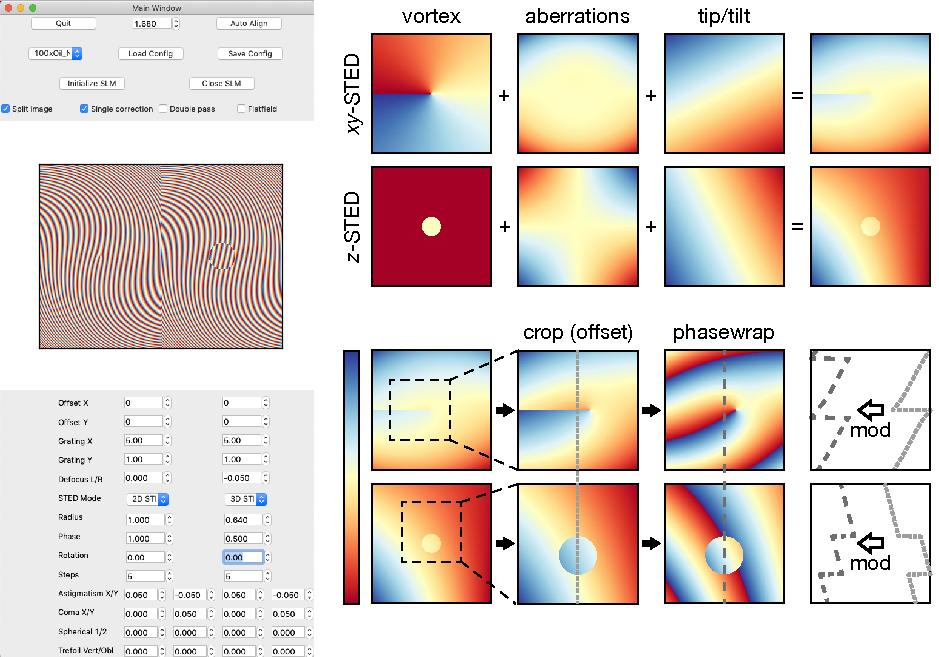
\includegraphics[width=\linewidth]{PatternGenerator.pdf}
			\caption{SLM control code.
				\emph{Left:} GUI main window.
				\emph{Top}: General controls to start/stop communication with SLM, select the objective and load/store configurations. 
				\emph{Center:} Preview of the SLM display.
				\emph{Bottom:} Controls to describe the pattern. 
				\newline
				\emph{Right:}
			}
			\label{fig:patterngen}
		\end{figure}
	
		The incident laser beam tends to drift continuously, \eg due to temperature fluctuations. 
		Therefore, the position of the phasemask with respect to the incident beam requires frequent realignment. 
		Thus, a responsive GUI and fast recalculation is especially important.
		To avoid computationally expensive re-calculation of the whole pattern as well as discontinuities at the edge of the patterns, all phasemasks are created at double the size required, and cropped to their actual size with a variable center position whenever the offset is changed. 
		With this design, the center position phasemask is quickly adjusted.
		
		The SLM can be run in single or split image geometry. 
		Change of SLM layout requires a restart of the code, and changing the boolean ``split image'' parameter in the \verb*|parameters_general.txt| file before restarting.
		The ``Flatfield'' checkbox activates addition of the flatfield correction image (see below).
		For a double-pass geometry, where the same laser beam bounces twice off the SLM, identical aberration correction is often needed for both passes. 
		Activating the ``single correction'' checkbox provides a convenient means to do so. 
		Likewise, activating the ``double pass'' checkbox duplicates and re-applies the flatfield correction (see below).
		
		Each of these SLM half-patterns is composed of several sub-patterns (\autoref{fig:patterngen}B):
		
		\emph{First,} the phase mask to create the different STED distributions.
		If left blank, a standard Gaussian focus was formed; vortex and top-hat pattern created the \emph{xy}-and \emph{z}-STED patterns. 
		Further, I implemented segmented (easy STED, \cite{Goerlitz2014}) and  bivortex phasemasks (coherent hybrid STED, \cite{Pereira2019}). 
		Full flexibility is provided by the options to enter python source code describing a pattern or uploading an image displaying the phase mask.
		
		\emph{Second,} aberration corrections are described via a weighted sum of Zernike polynomials. 
		While other parametrisations exist, Zernike polynomials are most widespread in the adaptive optics community because they are orthonormal, intuitive in their taxonomy and approximate the aberrations commonly encountered in microscopy with a finite subset \cite{Kubby2013book}. 
		
		\begin{equation}
			Z = \sum_{[0,0]}^{[m,n]}  a^{ \pm m}_n \cdot Z^{ \pm m}_n\left(\rho, \varphi\right)
		\end{equation}
		with
		\begin{equation}
			\begin{aligned}
				Z^{ m}_n\left(\rho, \varphi\right) &=& R^m_n\left(\rho\right)\cos\left(m\varphi\right)\\
				Z^{-m}_n\left(\rho, \varphi\right) &=& R^m_n\left(\rho\right)\sin\left(m\varphi\right)
			\end{aligned}
		\end{equation}
		and
		\begin{equation}
			R^m_n\left(\rho\right) = \sum^{\frac{n-m}{2}}_{k=0}\frac{\left(-1\right)^k\left(n-k\right)!}{k!\left(\frac{n+m}{2}-k\right)!\left(\frac{n-m}{2}-k\right)!}\rho^{n-2k}
		\end{equation}
		
		The weights of the most common aberrations (astigmatism, coma, spherical and trefoil) are accessible via the GUI.
		All others are implemented via their radial and azimuthal indices and are easily accessible via the source code window if needed.
		
		\emph{Third,} all patterns are created holographically to separate the first order from the undiffracted/unmodulated beam by adding a blazed grating \cite{Neil2000}. %check: is that the first paper suggesting this?
		Conveniently, this corresponds to tip and tilt of a mirror, implemented here as Zernike polynomials $Z^{-1}_1$ and $Z^{1}_1$.
		The holographic layout is further useful to align the position of the first diffraction order (\ie the STED beam focus) perfectly with the excitation beams \cite{Gould2013}, simply by changing the pitch of the grating slightly.
		
		\emph{Fourth,} a flatfield correction image can be loaded to correct for imperfections of the SLM surface (not shown in figure).
		If the SLM is operated in a double pass geometry, the flatfield correction is only imprinted on the polarization currently aligned with the SLM. 
		Therefore, an option is implemented to split the flatfield correction pattern and apply it again on the second half with the appropriate offset.
		
		In order to minimize computational time, and to keep the GUI responsive, I am storing all four subpatterns separately in the control PC's memory. 
		Whenever any of the parameters are changed the GUI, only the relevant subpatterns are updated and all subpatterns are added to compute the complete phasemask.
		Finally, the patterns are cropped to half their size to account for the offset, phasewrapped to unit brightness and scaled to match the SLM stroke to the wavelength of the STED beam.
	
	
	\section{Permanent parameter storage}
		
	
	\section{APGL Licence}
	Copyright (C) 2022 Wiebke Jahr
	
	This program is free software: you can redistribute it and/or modify it under the terms of the GNU Affero General Public License as published by the Free Software Foundation, either version 3 of the License, or (at your option) any later version.
	
	This program is distributed in the hope that it will be useful, but WITHOUT ANY WARRANTY; without even the implied warranty of	MERCHANTABILITY or FITNESS FOR A PARTICULAR PURPOSE.  See the GNU Affero General Public License for more details.
	
	You should have received a copy of the GNU Affero General Public License along with this program.  If not, see \href{https://www.gnu.org/licenses/}{https://www.gnu.org/licenses/}.
	
	% Booth lab SLM control SW. Never published?
	%https://github.com/jacopoantonello/slmtools
	
	
	\paragraph{Funding}
	W.J. gratefully acknowledges funding by a Human Frontier Science Program long term fellowship (HFSP LT000557/2018).
	\paragraph{Data Availability Statement}
	%TODO how does the python environment thingy work?
	All code is available under the following link:	\url{https://github.com/wiebkejahr}
	
	
	\printbibliography
	
\end{document}